\section{Theoretische Grundlage und Schematischer Aufbau des Versuches}
\label{sec:Theorie}
Ziel des Versuches ist es den glühelektrischen Effekt genauer zu untersuchen. Dafür soll die Austrittsarbeit von Wolfram bestimmt und deren Temperaturabhängigkeit nachvollzogen werden. 

Um eine Wechselwirkung der freien Elektroen mit den Gasmolekühlen zu verhindern wird das Experiment im Hochvakuum durchgeführt. Der schematische Aufbau ist in Abbildung \ref{fig:SHD} zu sehen. 

\begin{figure}
  \centering
  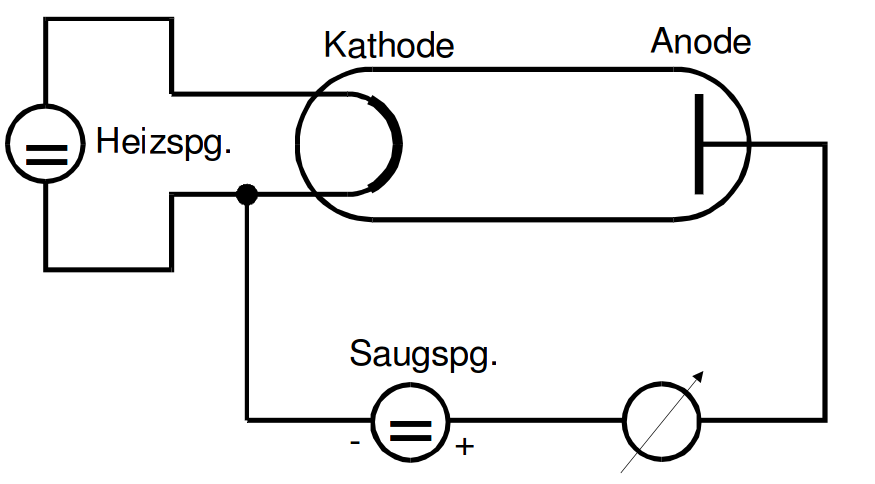
\includegraphics[height=5cm]{picture/Diode.png}
  \caption{Schaltung einer Hochvakuum-Diode \cite{pra}}
  \label{fig:SHD}
\end{figure}

Die Kathode wird durch einen Heizstrom $I_\text{H}$ erhitzt und die dadurch freigesetzten Elektronen mittels einer $U_B$ Beschleunigungsspannung Richtung Anode abgesaugt. Der zwischen den Anode und Katode fließende Strom $I_\text{S}$ wird in einem Diagramm gegen die Beschleunigungsspannung aufgetragen (siehe Abbildung \ref{fig:Ken}) und die Kennlinie in drei Gebiete eingeteilt.
\begin{figure}
  \centering
  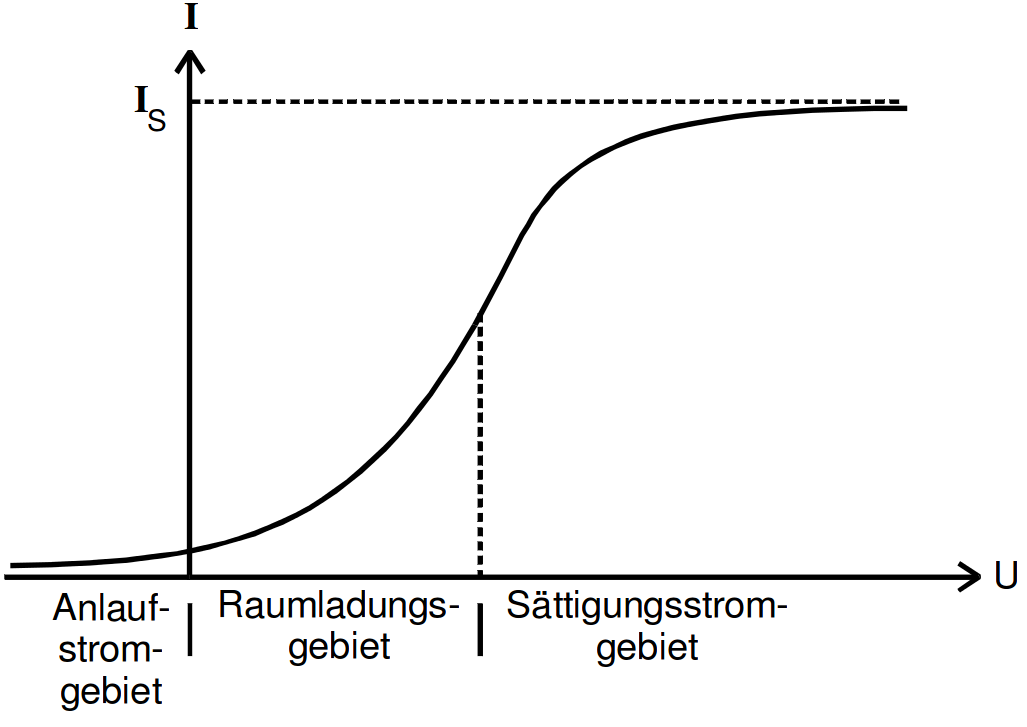
\includegraphics[height=5cm]{picture/Kennlinie.png}
  \caption{Kennlinie \cite{pra}}
  \label{fig:Ken}
\end{figure}
Das Gebiet wo eine kleine Gegenspannung angelegt wird, wird als Anlaufstromgebiet bezeichnet. Der Strom $I_\text{S}$ ist darauf zurückzuführen das die aus der Kathode austretenden Elektroden eine statistisch verteilte Bewegungsenergie besitzen die ausreicht die Gegenspannung zur Anode zu überwinden. Die Stromdichte berechnet sich in Abhängigkeit der Temperatur nach:
\begin{equation}
  j(V) = j_0 exp\left( - \frac{e_0 V}{k_\text{B}}T \right)
  \label{eqn:jv}
\end{equation}
Anschließend an das Anlaufstromsgebiet befindet sich das Raumladungsgebiet. Es ist dadurch gekennzeichnet das nicht alle Elektronen von Feld abgezogen werden und einige der Feldlinien bereits vor der Kathode enden. Dies geschieht da die Raumladungsdichte aufgrund der Bewegung der Elektronen abnimmt. 
\begin{equation}
  j = \rho v
  \label{eqn:j}
\end{equation}
Daher muss das ohmsche Gesetz in diesem Bereich durch das Langmuir-Schottkysche Raumladungsgesetz 
\begin{equation}
  j = \frac{4}{9}\varepsilon_0\sqrt{2e_0/m_0}\frac{V^{3/2}}{a^2}
  \label{eqn:jLS}
\end{equation}
ersetzt werden. Ziel des Versuches ist es die Beziehung j \propto $V^{3/2}$ zu bestätigen.
An das Raumladungsgebiet schließt sich das Sättigungsgebiet an. Dabei erreichen alle  Elektronen die Katode verlassen die Anode. Der Sättigungsstrom sollte nun durch die Richardson-Gleichung beschriebenwerden und  noch von der Austrittsarbeit sowie der Temperatur abhängen.
\begin{equation}
  j_\text{s} (T) = 4 \pi \frac{e_0 m_0 k_\text{b}^2}{h^3} T^2 exp \left( \frac{-e_0 \Phi}{k_\text{B} T} \right)
  \label{eqn:js}
\end{equation}
\subsection{Fehlerrechnung}
Sämtliche Fehlerrechnungen werden mit Hilfe von Python 3.4.3 durchgeführt.
\subsubsection{Mittelwert}
Der Mittelwert einer Messreihe $x_\text{1}, ... ,x_\text{n}$ lässt sich durch die Formel
\begin{equation}
	\overline{x} = \frac{1}{N} \sum_{\text{k}=1}^\text{N} x_k
	\label{eqn:ave}
\end{equation}
berechnen. Die Standardabweichung des Mittelwertes beträgt
\begin{equation}
	\Delta \overline{x} = \sqrt{ \frac{1}{N(N-1)} \sum_{\text{k}=1}^\text{N} (x_\text{k} - \overline{x})^2}
	\label{eqn:std}
\end{equation}

\subsubsection{Gauß'sche Fehlerfortpflanzung}
Wenn $x_\text{1}, ..., x_\text{n}$ fehlerbehaftete Messgrößen im weiteren Verlauf benutzt werden, wird der neue Fehler $\Delta f$ mit Hilfe der Gaußschen Fehlerfortpflanzung angegeben.
\begin{equation}
	\Delta f = \sqrt{\sum_{\text{k}=1}^\text{N} \left( \frac{ \partial f}{\partial x_\text{k}} \right) ^2 \cdot (\Delta x_\text{k})^2}
	\label{eqn:var}
\end{equation}

\subsubsection{Lineare Regression}
Die Steigung und y-Achsenabschnitt einer Ausgleichsgeraden werden gegebenfalls mittels Linearen Regression berechnet.
\begin{equation}
	y = m \cdot x + b
	\label{eqn:reg}
\end{equation}
\begin{equation}
	m = \frac{ \overline{xy} - \overline{x} \overline{y} } {\overline{x^2} - \overline{x}^2}
	\label{eqn:reg_m}
\end{equation}
\begin{equation}
	b = \frac{ \overline{x^2}\overline{y} - \overline{x} \, \overline{xy}} { \overline{x^2} - \overline{x}^2}
	\label{eqn:reg_b}
\end{equation}
